\newpage
\section{Physical Layer}
\subsection{Arten der Kommunikation (Verkehrsbeziehung)}{
    \begin{itemize}[noitemsep]
        \item Simplex $\to$ Ein Kanal, in eine Richtung
        \item Halbduplex $\to$ Ein Kanal, abwechslungsweise in zwei Richtungen
        \item Vollduplex $\to$ Ein Kanal pro Richtung
    \end{itemize}
}
\subsection{Arten der Verbindungen (Kopplung)}

\paragraph{Punkt - Punkt}{

    {Direkte Verbindung zweier Kommunikationspartner }

    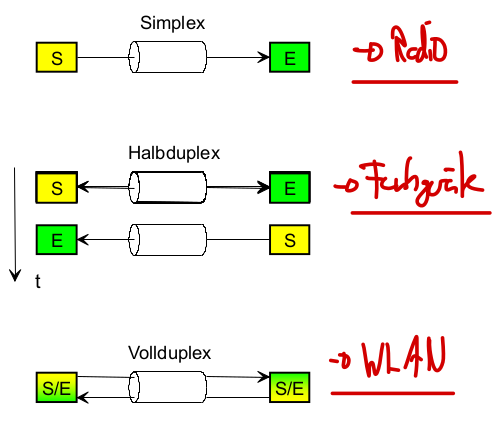
\includegraphics[scale=.35]{img/kopplung.png}
}

\paragraph{Shared Medium }{
    {Mehrere Partner verwenden das gleiche Medium   \\}

    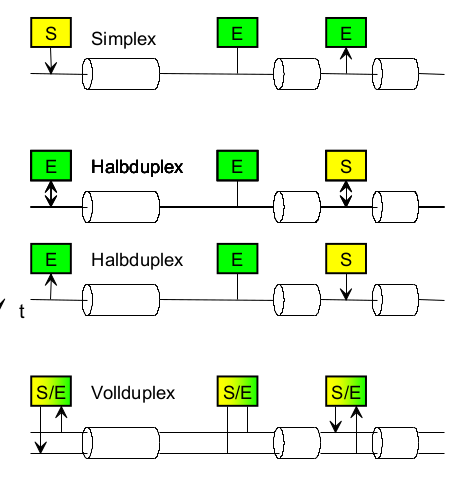
\includegraphics[scale=.35]{img/kopplung_2.png}

}
\vfill\null
\columnbreak
\subsection{Leitungscodes}{
    Leitungscodes sollen:

    \begin{itemize}[noitemsep]
        \item die physikalisch vorhandene Bandbreite effizient nutzen
        \item Taktrückgewinnung erlauben, um eine separate Taktleitung einzusparen
        \item möglichst gleichspannungsfrei sein, um Sender und Empfänger mit Übertragern (Signaltransformatoren, Magnetics) galvanisch trennen zu können.
    \end{itemize}

    Beispiele:
    \begin{itemize}[noitemsep]
        \item 3-wertiger AMI-Code (Alternate Mark Inversion)
        \item PAM3 Kanalcodierung
    \end{itemize}
}

\subsection{Serielle asynchrone Übertragung}{

    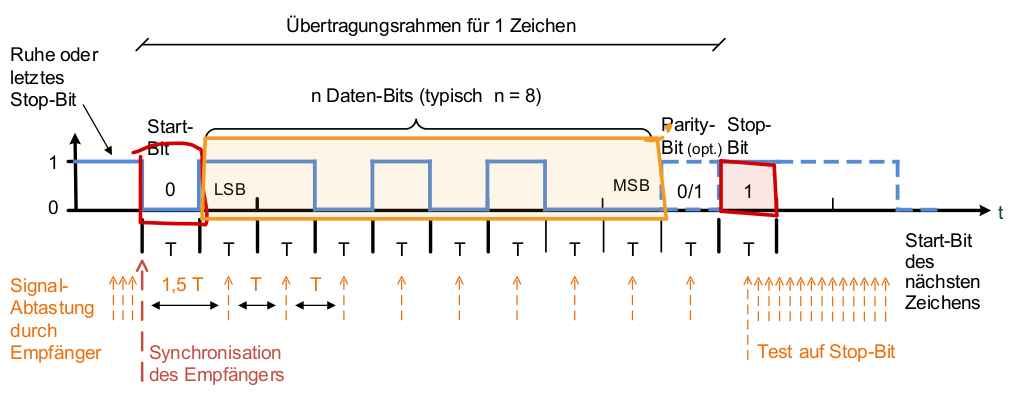
\includegraphics[scale=.25]{img/async.png}
    {$LSB$ = Least Significant Bit, $MSB$ = Most Significant Bit}\\

    \begin{tikzpicture}
        \node [examplebox] (box){
            \begin{minipage}{0.3\textwidth}
                Übertragener Wert ablesen: \\
                $LSB$ zuerst, $MSB$ zuletzt \\
                $  1101`0100 \to LSB $ zuerst $ \to 0100`1101 $
            \end{minipage}
        };
        \node[exampletitle, right=8pt] at (box.north west) {Wichtig:};
    \end{tikzpicture}


}



\subsection{Serielle synchrone Übertragung}{
    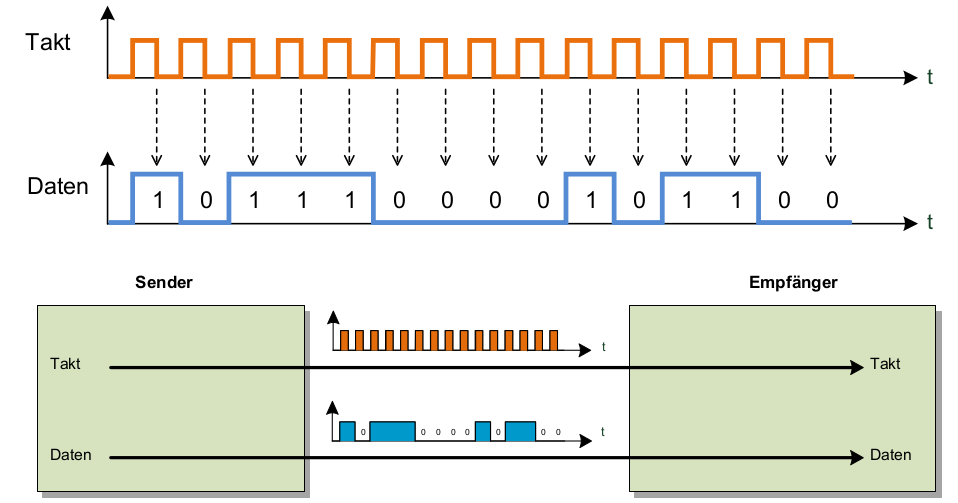
\includegraphics[scale=.275]{img/sync.png}
}

\columnbreak
\subsection{Datenübertragungsrate}{
    \begin{itemize}[noitemsep]
        \item Baudrate $\to$ Symbole pro Sekunde
        \item Zeichenrate $\to$ Zeichen pro Sekunde
    \end{itemize}
}

\subsection{Frequenz}{
    {Die Frequenz ist die Anzahl der Schwingungen pro Sekunde.\\
            Masseinheit Hertz (Hz)\\}
}

\subsection{Bit-Dauer }
{  T [s] = Bit-Dauer, B = Baud \\}
$$ T = \frac{1}{B}$$


\subsection{maximale Symbolrate}
{    Die maximale Symbolrate $f_s$ (Baud) ist gleich der doppelten Bandbreite B (Hz) des
    Übertragungskanals.
}
{Einheit: Baud (Bd)}

{Nyquist:}
$$ f_s = 2 \cdot B$$

\subsection{Maximal erreichbare Bitrate}{
R [bit/s] = Bitrate \\
$$ R \leq 2B \cdot log_2{M} $$
$$ log_2(x) = \frac{log_{10}(x)}{log_{10}(2)} $$
}



\subsection{Bandbreite}{
    Die Bandbreite hängt von der Übertragungsstrecke und der Stärke des Signals im
    Vergleich zu den vorhandenen Störungen, ab.
    \begin{itemize}[noitemsep]
        \item Eigenschaft des Übertragungskanals und durch das Medium begrenzt
        \item Masseinheit Hertz (Hz)
    \end{itemize}
}

\subsection{Kanalkapazität}{
    Berücksichtigt für einen realen Kanal das Signal-zu-Rausch Leistungverhältnis S/N (Shannon)
    \\ Einheit Bit/s (bps)
    $$ C_s = B \cdot log_2(1 + \frac{S}{N})$$
    $$ log_2(x) = \frac{log_{10}(x)}{log_{10}(2)} $$
}
